\documentclass[12pt]{memoir}
\usepackage[backend=bibtex,style=ieee,doi=false,url=false,isbn=false]{biblatex}
\usepackage[pdftex]{graphicx}
\usepackage{enumitem}
\usepackage{url}
\usepackage{style}

\addbibresource{references}

\title{}
\author{Andrew Head}

\begin{document}

\definition{Title}{Supporting Systematic Code Inspection During Opportunistic Programming}

\definition{Author}{Andrew Head, PhD Student, UC Berkeley}

Clarke~\cite{clarke_what_2007} introduced the persona of an \emph{opportunistic developer} to describe a software developer who writes code in an ``exploratory fashion'' and develops a ``sufficient understanding of a technology to understand how it can solve a business problem''.
(This contrasts with the \emph{systematic developer}, who writes code defensively and ``develops a deep understanding of a technology before using it''~\cite{clarke_what_2007}.)
In their study of exhibit designers at San Francisco's Exploratorium interactive science museum, Brandt et al.\ reported on a group who engaged in \emph{opportunistic programming} who weren't professional developers~\cite{brandt_opportunistic_2008} but were very much what might be considered as end-user programmers --- those developing code for personal rather than public use~\cite{ko_state_2011}.

Brandt et al.\ associated several habits with opportunistic programming that are counter to what we would hope for students working with code or end-users developing a better understanding of code.
Those programming opportunistically likely to incorporate functionality by copying and pasting code, often from online sources~\cite{brandt_two_2009}.
They are more likely to implement functionality from scratch for well-known libraries, instead of reusing existing systems and libraries~\cite{brandt_opportunistic_2008}.
They also practice ``code satisficing'', implementing functionality in a sub-optimal way in order to maintain flow and move on to other functionality~\cite{brandt_opportunistic_2008}.

While opportunistic programming is powerful in that it allows one to rapidly prototype and ideate and that it reduces the cycle time of editing and debugging code~\cite{brandt_opportunistic_2008}, this behavior discourages the formation of new mental models and an introduction to new tools that should be encouraged for both novice programmers and many end-user programmers.
The author of this proposal observed much of what would be called ``opportunistic'' habits while instructing a user interface design course.
After providing reference code to students for programming interfaces on Android phones and smartwatches, he helped students debug problems related to API reuse and the side effects of mixed code from multiple examples after hearing students self-report to having ``copied and pasted'' code from online tutorials and the slides he distributed.
In light of a prevalence of the ease of opportunistic habits and programmers' ability to copy-and-paste code from an increasingly comprehensive body of crowd documentation online~\cite{parnin_crowd_2012}, I define the goals of my research:

\emph{In my research, I develop and study software artifacts to support systematic inspection of found code from information interfaces programmers use when developing opportunistically.}

The theoretical deliverables of this work is establishing how systematic habits amidst opportunistic practice will improve:
(\emph{a}) programmers' mental models of reused code, libraries and tools used they develop
(\emph{b}) enable more accurate feasibility assessments of upcoming tasks (for example, see~\cite{ko_role_2011})
(\emph{c}) reduce design barriers~\cite{ko_six_2004} when planning new functionality

The artifacts that I develop belong to two themes:
\begin{itemize}[noitemsep]
\item Techniques for automatically generating instructive explanations and demonstrations of found code
\item Interfaces for critical inspection of alternatives when selecting code for reuse
\end{itemize}

I have developed the artifacts that enable exploration within both of these themes, and published a first paper on the first of the two themes.
Toward the first, a paper I presented at VL/HCC explored techniques for automatically augmenting code in online examples with natural languages explanations and demonstrations of code.\footnote{%
The Tutorons system was implemented as both a browser plugin and a standalone JavaScript library, and can be viewed in action on \url{www.tutorons.com}.
}
We put forward a set of four guidelines to inspire the development of context-sensitive help:
(\emph{a}) leverage multiple representations to illuminate high-level intent and enable low-level understanding of syntax
(\emph{b}) be concise --- skip static explanations and focus on dynamically generated content
(\emph{c}) reappropriate existing documentation
(\emph{d}) inspect code examples on a large scale to support explanations of common usage.
In a nine-participant user study, the system was shown to reduce the number of accesses to external documentation needed to modify online code to perform new tasks.
\textbf{Next steps will include \ldots}

Towards the second goal, I and co-developer have built a visual search interface for StackOverflow, a popular online programming Q\&A.
In response to Brandt et al.'s recommendations to develop tools that support ``comparing, reasoning about, integrating, and modifying found code''~\cite{brandt_opportunistic_2008}, we developed StackSkim, \emph{a visual search interface for exploring answers to StackOverflow questions that have a multitude of answers}.
The interface offers rapid visual inspection of frequent libraries used for addressing the searcher's programming problem;
through direct manipulation, users can also rapidly collect and compare similar code snippets.
\textbf{Next steps will include \ldots}

\begin{figure}%
  \centering
  \parbox{.45\textwidth}{%
    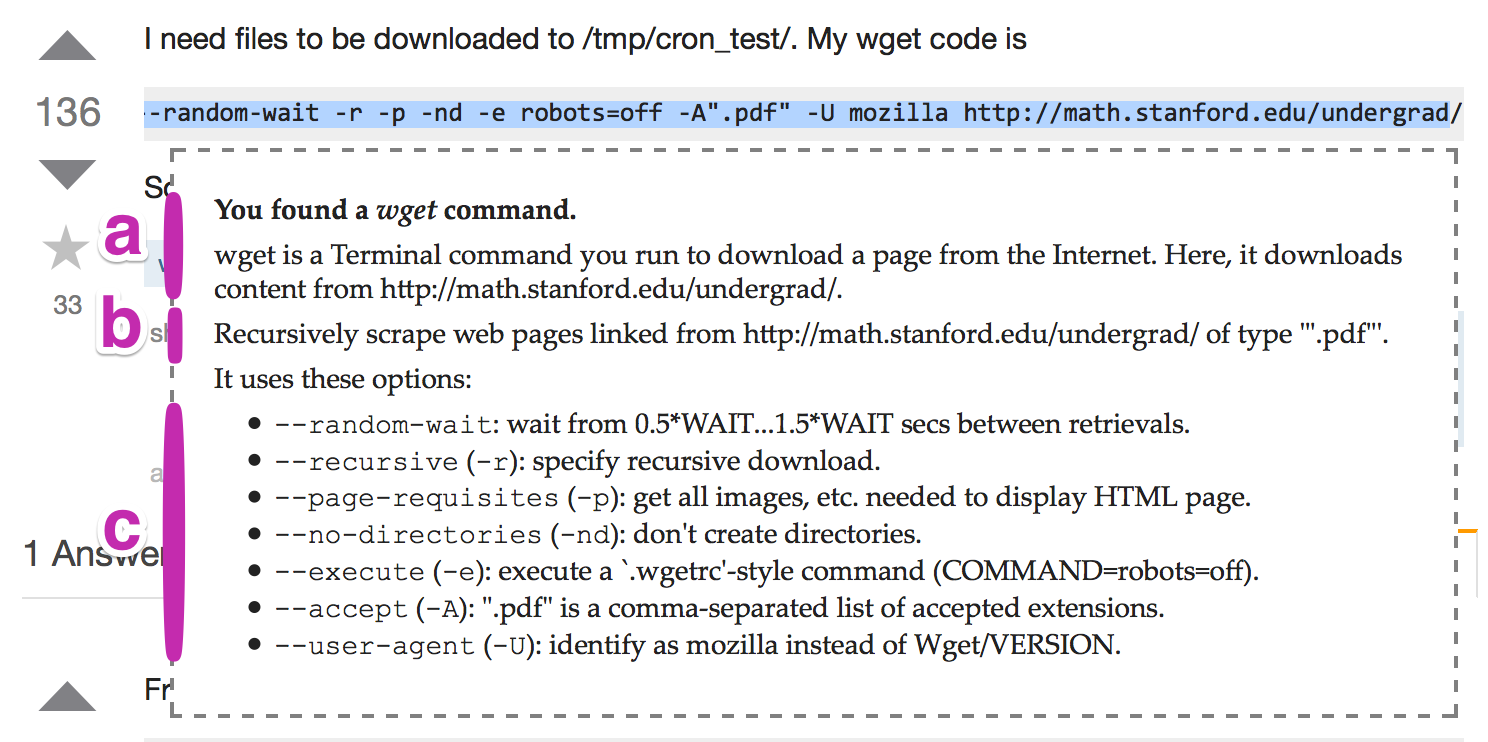
\includegraphics[width=\linewidth]{figures/tutorons_microexplanation}
    \caption{%
      A micro-explanation for a command line generated by a Tutoron with multiple levels of detail 
      (definition, high-level intent, arguments)
    }\label{fig:tutorons_microexplanation}
  }%
  \qquad
  \parbox{.45\textwidth}{%
    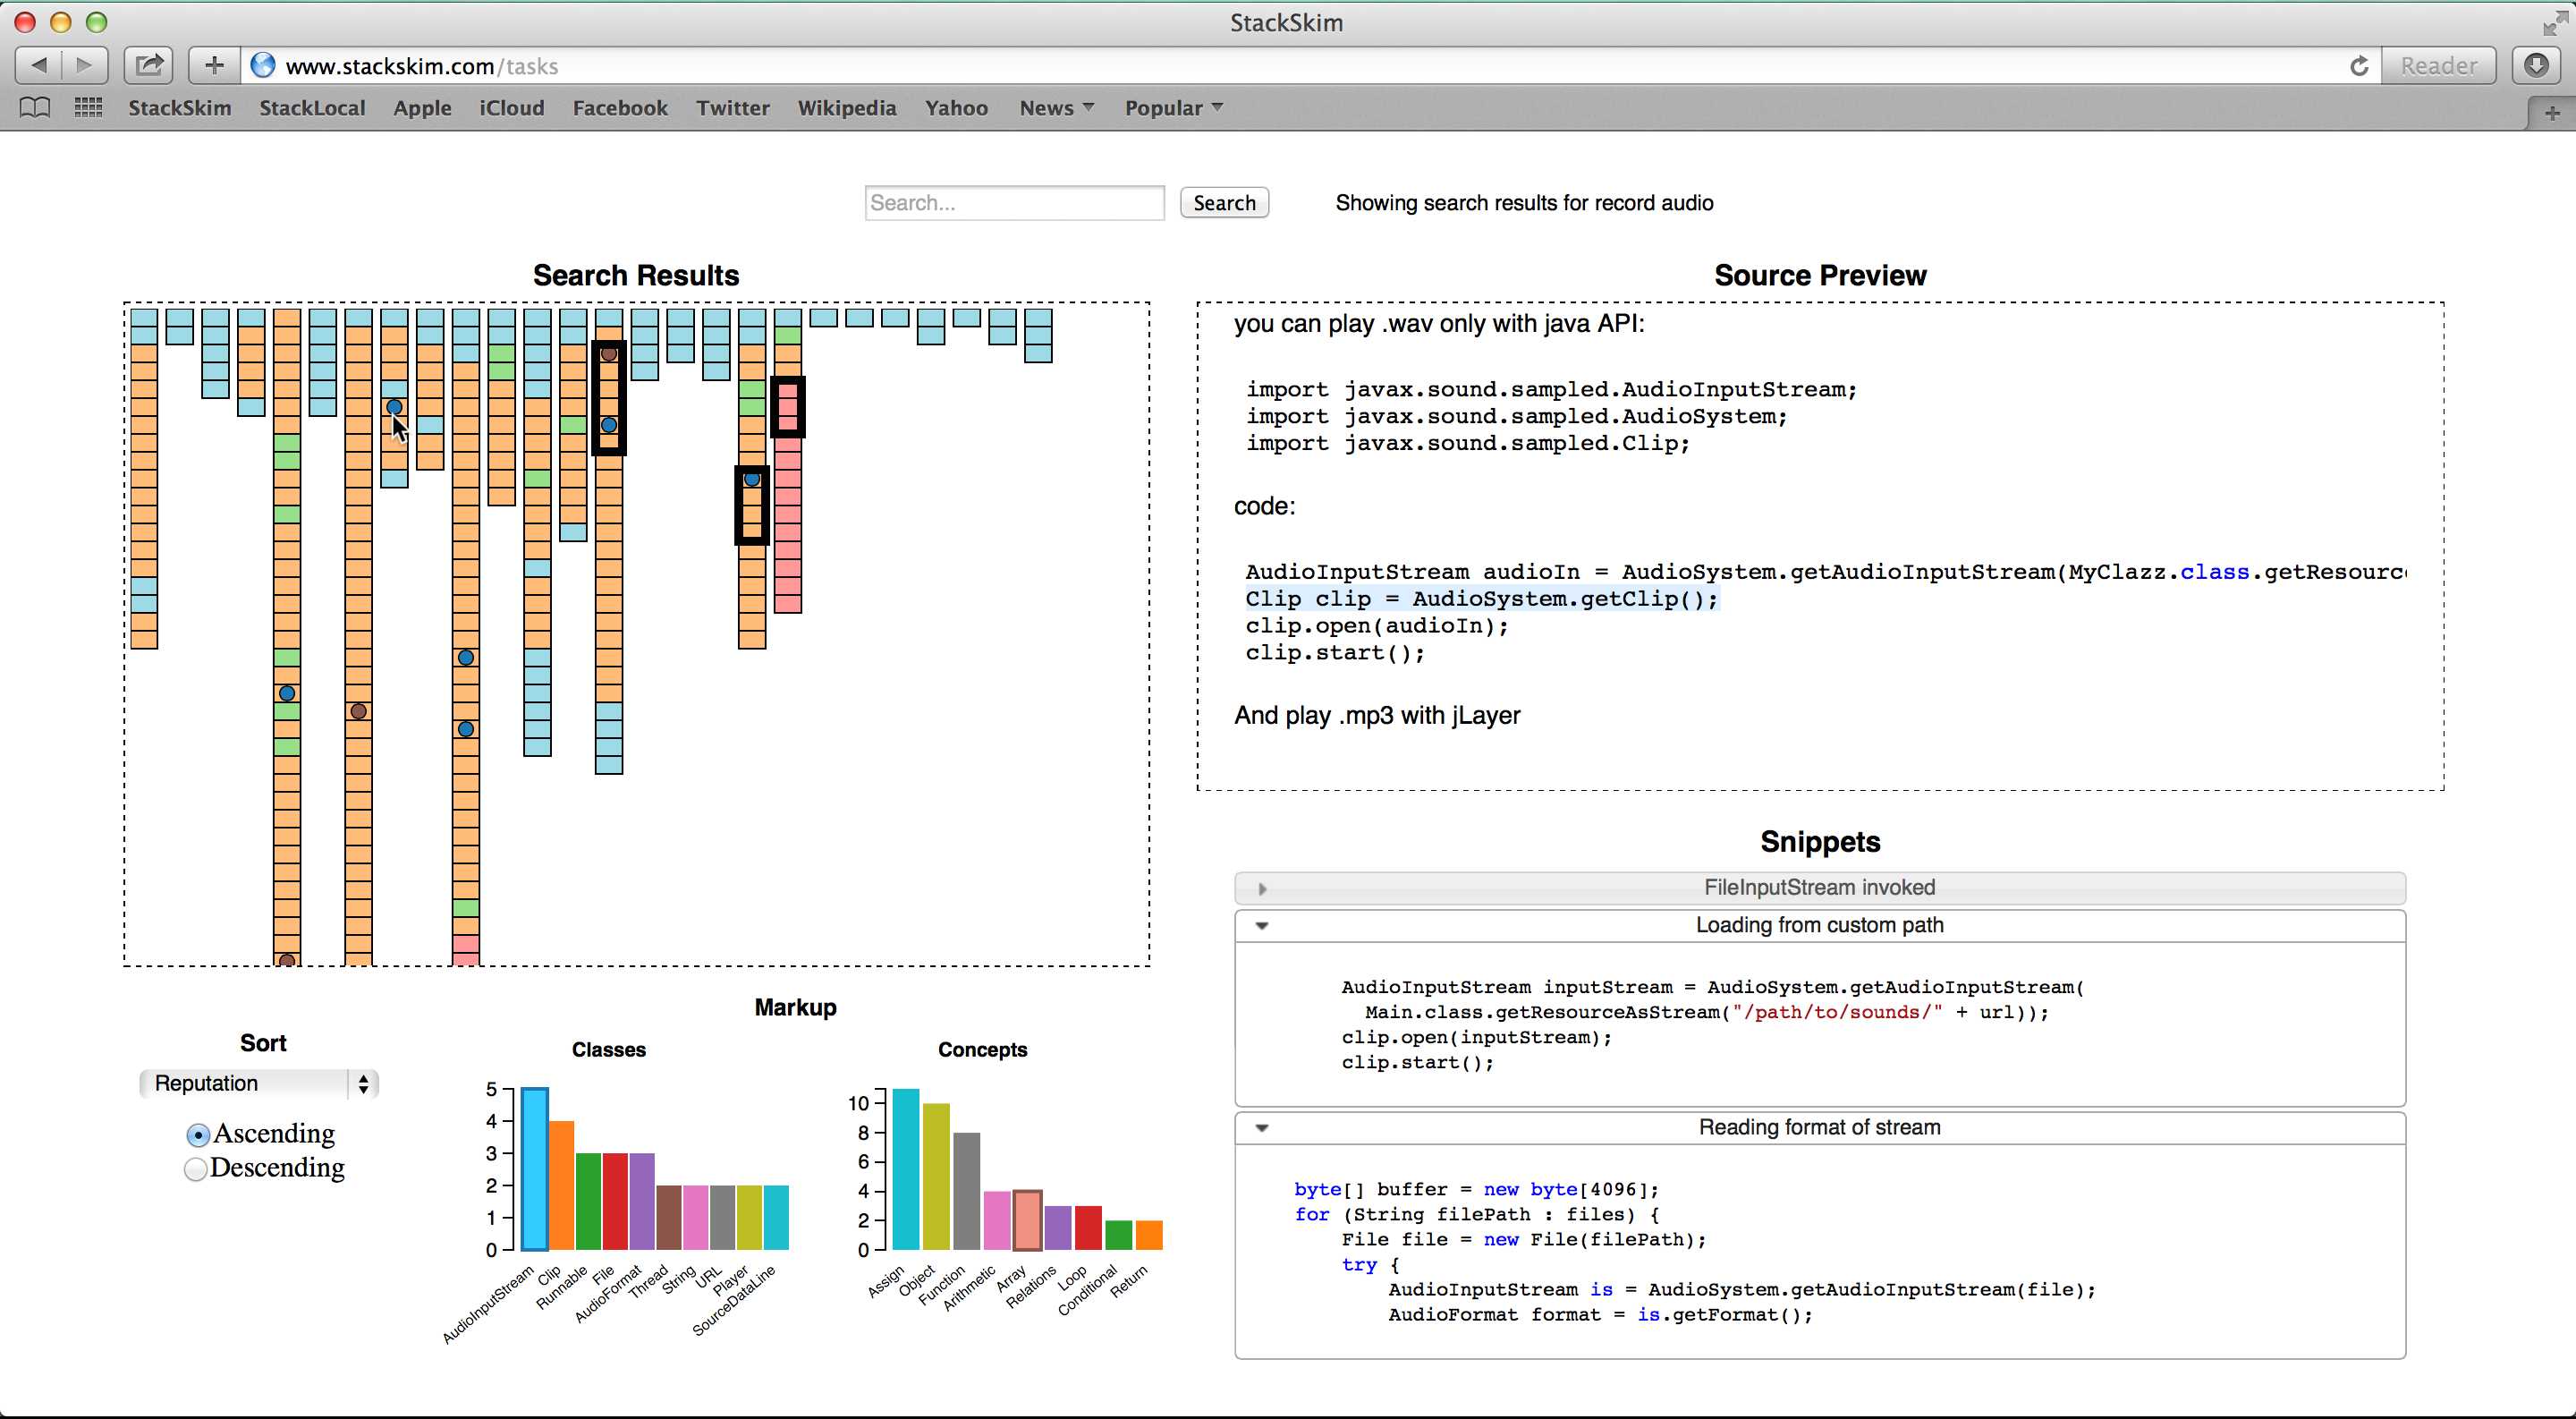
\includegraphics[width=\linewidth]{figures/stackskim_ui}
    \caption{%
      StackSkim, a visual interface for comparing and noticing trends in large collections of code examples that solve the same problem.
    }\label{fig:stackskim_ui}
  }
\end{figure}

Each of these efforts relies on the cultivation of new software artifacts to aid programmers in understanding code during an opportunistic programming task.
Each has already followed and will continue to follow a mixed methods approach of observation and controlled experiments to determine how these tools indeed alter not only the task of opportunistic programming, but also programmers' behavior in selecting, understanding, and using code found online.
We are currently developing a version of Tutorons explanations that we hope will be incorporated into an introductory CS classroom's online textbook to better understand the role of automatic explanations of code for novice programmers.

\section{References}
\printbibliography[heading=none]

\end{document}
